% ------------------------------------------------------------------------
% ------------------------------------------------------------------------
% Modelo de Artigo Acadêmico
% Em conformidade com:
% ABNT NBR 6022:2018: Informação e Documentação - Artigo em Publicação Periódica Científica - Apresentação
%
% Adaptado para:
% SEPA: Seminário Estudantil de Produção Acadêmica da UNIFACS
%
% Baseado na Biblioteca abnTeX2 v1.9.7
% ------------------------------------------------------------------------
% ------------------------------------------------------------------------
\documentclass[
	% Opções da classe memoir
	article,			    % indica que é um artigo acadêmico
	12pt,				    % tamanho da fonte
	oneside,			    % para impressão apenas no recto. Oposto a twoside
	a4paper,			    % tamanho do papel. 
	% Opções da classe abntex2
	chapter=TITLE,		    % títulos de capítulos convertidos em letras maiúsculas
	section=TITLE,		    % títulos de seções convertidos em letras maiúsculas
	subsection=TITLE,	    % títulos de subseções convertidos em letras maiúsculas
	%subsubsection=TITLE    % títulos de subsubseções convertidos em letras maiúsculas
	% Opções do pacote babel
	english,			    % idioma adicional para hifenização
	brazil,				    % o último idioma é o principal do documento
	sumario=tradicional
]{abntex2}
% ------------------------------------------------------------------------
% PACOTES
% ------------------------------------------------------------------------
% Pacotes fundamentais 
\usepackage{times}			    % Usa a fonte Times New Roman
\usepackage[T1]{fontenc}		% Selecao de codigos de fonte.
\usepackage[utf8]{inputenc}		% Codificacao do documento (conversão automática dos acentos)
\usepackage{indentfirst}		% Indenta o primeiro parágrafo de cada seção.
\usepackage{nomencl} 			% Lista de simbolos
\usepackage{color}				% Controle das cores
\usepackage{graphicx}			% Inclusão de gráficos
\usepackage{microtype} 			% Para melhorias de justificação
% Pacotes adicionais, usados apenas no âmbito do Modelo Canônico do abnteX2
\usepackage{lipsum}				% Para geração de dummy text
% Pacotes de citações
\usepackage[brazilian,hyperpageref]{backref}	 % Paginas com as citações na bibliografia
\usepackage[alf,bibjustif,abnt-emphasize=bf,abnt-etal-text=emph]{abntex2cite}  % Citações padrão ABNT, forçar a justificação da bibliografia e enfatizar com negrito
% Pacotes extras 
\usepackage{fancyhdr}           % Personalização do cabeçalho e rodapé
\usepackage[final]{listings}    % Personalização de código
\lstset{language=C}
% ------------------------------------------------------------------------
% CONFIGURAÇÃO DOS PACOTES
% ------------------------------------------------------------------------
% Configurações do pacote backref
% Usado sem a opção hyperpageref de backref
\renewcommand{\backrefpagesname}{Citado na(s) página(s):~}
% Texto padrão antes do número das páginas
\renewcommand{\backref}{}
% Define os textos da citação
\renewcommand*{\backrefalt}[4]{
	\ifcase #1
		Nenhuma citação no texto.
	\or
		Citado na página #2.
	\else
		Citado #1 vezes nas páginas #2.
	\fi
}
% Configuração dos nomes padrões do babel
%\addto\captionsbrazil{
%    \renewcommand{\bibname}{Referências Bibliográficas}
%}
% Configuração do título das referências (anteriormente modificado)
\renewcommand{\bibsection}{%
    \section*{\bibname}
    \bibmark
    \ifnobibintoc\else
        \phantomsection
    \fi
    \prebibhook
}
% Modificando o tamanho da fonte "large" que é 14.4pt, para 14pt
%\renewcommand{\large}{\fontsize{14}{14}\selectfont}
% ------------------------------------------------------------------------
% DADOS DO DOCUMENTO
% ------------------------------------------------------------------------
% Informações de dados para capa
\autor{\normalsize{\textbf{Felipe Rios da Silva Cordeiro}}}
\instituicao{
    UNIFACS - UNIVERSIDADE SALVADOR
    ESCOLA DE ARQUITETURA, ENGENHARIA\\ E TECNOLOGIA DA INFORMAÇÃO
    BACHARELADO EM ENGENHARIA DA COMPUTAÇÃO
}
\titulo{\uppercase{\normalsize{\textbf{EXECUÇÃO ESPECULATIVA:\\
LIMITES DA EXPLORAÇÃO DE INFORMAÇÕES SENSÍVEIS}}}}
\local{Salvador}
%\data{2019}
\tipotrabalho{Trabalho de Conclusão de Curso, Graduação}
\preambulo{Trabalho de conclusão de curso apresentado ao curso de graduação em Engenharia da Computação da Universidade Salvador - UNIFACS, como requisito fundamental para obtenção do título de Engenheiro da Computação.}
\orientador[Orientador:]{\normalsize{\textbf{Éldman de Oliveira Nunes}}}
%\tituloestrangeiro{Canonical article template in \abnTeX: optional foreign title}
% ------------------------------------------------------------------------
% META DADOS DO PDF
% ------------------------------------------------------------------------
% Alterando o aspecto da cor azul
\definecolor{blue}{RGB}{41,5,195}
% Informações do PDF
\makeatletter
\hypersetup{
 	%pagebackref=true,
	pdftitle={\@title}, 
	pdfauthor={\@author},
	pdfsubject={\imprimirpreambulo},
    pdfcreator={LaTeX with abnTeX2 and Overleaf},
	pdfkeywords={abnt}{latex}{abntex}{abntex2}{atigo científico}, 
	colorlinks=false,       % false: boxed links; true: colored links
	linkcolor=blue,         % color of internal links
	citecolor=blue,        	% color of links to bibliography
	filecolor=magenta,      % color of file links
	urlcolor=blue,
	bookmarksdepth=4
}
\makeatother
% ------------------------------------------------------------------------
% CONFIGURAÇÕES DAS FOLHAS E AJUSTES NAS FONTES GERAIS
% ------------------------------------------------------------------------
% Compila o índice
\makeindex
% Altera as margens
\setlrmarginsandblock{3cm}{2cm}{*}
\setulmarginsandblock{3cm}{2cm}{*}
\checkandfixthelayout
% Espaçamentos entre linhas e parágrafos 
% O tamanho do parágrafo é dado por (espaçamento na primeira linha):
\setlength{\parindent}{1.25cm}
% O espeçamento padrão é definido como \OnehalfSpacing, ou seja, um espaço e meio conforme estabelece a ABNT NBR 14724:2011
% ------------------------------------------------------------------------
% CABEÇALHOS E RODAPÉS
% ------------------------------------------------------------------------
% Criar um novo estilo de cabeçalhos e rodapés
\pagestyle{fancy}
%\setlength{\headheight}{80pt}
\fancyhf{}
%\lhead{\includegraphics[width=0.4\textwidth]{/images/image00.png}}
%\rhead{
%{\fontsize{8}{1.5}\selectfont
%\begin{vplace}
%TCC - TRABALHO DE CONCLUSÃO DE CURSO\break
%COORDENAÇÂO DE ENGENHARIA DA COMPUTAÇÃO\end{vplace}}}
\fancypagestyle{plain}{
    \renewcommand{\headrulewidth}{0pt}
    \renewcommand{\footrulewidth}{0pt}
    \fancyhfoffset[LE]{0mm}
    \fancyhfoffset[RE]{0mm}
    \fancyhfoffset[LO]{0mm}
    \fancyhfoffset[RO]{0mm}
}
% ------------------------------------------------------------------------
% CAPÍTULOS, SEÇÕES E SUBSEÇÕES
% ------------------------------------------------------------------------
% Chapter 12pt + Bold
\renewcommand{\ABNTEXchapterfont}{\bfseries}
\renewcommand{\ABNTEXchapterfontsize}{\normalsize}
% Section 12pt + Bold
\renewcommand{\ABNTEXsectionfont}{\bfseries}
\renewcommand{\ABNTEXsectionfontsize}{\normalsize}
% SubSection 12pt
\renewcommand{\ABNTEXsubsectionfont}{\normalfont}
\renewcommand{\ABNTEXsubsectionfontsize}{\normalsize}
% SubSubSection 12pt + Bold + Underline
\renewcommand{\ABNTEXsubsubsectionfont}{\bfseries}
\renewcommand{\ABNTEXsubsubsectionfontsize}{\normalsize}
\setsubsubsecheadstyle{\ABNTEXsubsubsectionfont\ABNTEXsubsubsectionfontsize\ABNTEXsubsubsectionupperifneeded\coloruline[black]}
% SubSubSubSection 12pt + Lowercase
\setparaheadstyle{\normalfont\ABNTEXsubsubsectionfont\ABNTEXsubsubsectionfontsize}
% Retirando espaçamentos antes dos capítulos
\setlength{\beforechapskip}{\baselineskip}
% Retirando espaçamentos depois dos capítulos
\setlength{\afterchapskip}{\baselineskip}
% Recriando a variável que instancia o resumo
\renewenvironment{resumoumacoluna}{}

% ------------------------------------------------------------------------
% INÍCIO DO DOCUMENTO
% ------------------------------------------------------------------------
\begin{document}
% Seleciona o idioma do documento (conforme pacotes do babel)
%\selectlanguage{english}
\selectlanguage{brazil}
% Retira espaço extra obsoleto entre as frases.
\frenchspacing 
% ------------------------------------------------------------------------
% ELEMENTOS PRÉ-TEXTUAIS
% ------------------------------------------------------------------------
\pretextual
\pagestyle{fancy}
% página de titulo principal (obrigatório)
%\maketitle
\begin{SingleSpace}
    \begin{center}
        \imprimirtitulo
    \end{center}
    \begin{flushright}
        \imprimirautor
        \footnote{Graduando em Engenharia da Computação, UNIFACS. E-mail: felipe.rios.silva@outloook.com}
        \\
        \imprimirorientador
        \footnote{Docente Orientador Doutor em Processamento Digital de Imagens, UNIFACS. E-mail: eldman.nunes@unifacs.br}
    \end{flushright}
\end{SingleSpace}
% Titulo em outro idioma (opcional)
% Resumo em Português
\begin{resumoumacoluna}
    \footnotesize{\begin{SingleSpace}
        \noindent
        \textbf\resumoname\\
        Conforme a ABNT NBR 6022:2018, o resumo no idioma do documento é elemento obrigatório. Constituído de uma sequência de frases concisas e objetivas e não de uma simples enumeração de tópicos, não ultrapassando 250 palavras, seguido, logo abaixo, das palavras representativas do conteúdo do trabalho, isto é, palavras-chave e/ou descritores, conforme a NBR 6028. (\ldots) As palavras-chave devem figurar logo abaixo do resumo, antecedidas da expressão Palavras-chave:, separadas entre si por ponto e finalizadas também por ponto.\\\\
        \textbf{Palavras-chave:} latex. abntex. editoração de texto.
        \vspace{\onelineskip}
    \end{SingleSpace}}
\end{resumoumacoluna}
% Resumo em Inglês
\renewcommand{\resumoname}{Abstract}
\begin{resumoumacoluna}
    \footnotesize{\begin{SingleSpace}
        \begin{otherlanguage*}{english}
            \noindent
            \textbf\resumoname\\
            Conforme a ABNT NBR 6022:2018, o resumo no idioma do documento é elemento obrigatório. Constituído de uma sequência de frases concisas e objetivas e não de uma simples enumeração de tópicos, não ultrapassando 250 palavras, seguido, logo abaixo, das palavras representativas do conteúdo do trabalho, isto é, palavras-chave e/ou descritores, conforme a NBR 6028. (\ldots) As palavras-chave devem figurar logo abaixo do resumo, antecedidas da expressão Palavras-chave:, separadas entre si por ponto e finalizadas também por ponto.\\\\
            \textbf{Keywords:} latex. abntex.
        \end{otherlanguage*}
    \end{SingleSpace}}
\end{resumoumacoluna}
% ------------------------------------------------------------------------
% ELEMENTOS TEXTUAIS
% ------------------------------------------------------------------------
\textual
\pagestyle{fancy}
% ------------------------------------------------------------------------
% INTRODUÇÃO
% ------------------------------------------------------------------------
\section{Introdução}
% ---------------------------------
% TEMA
% ---------------------------------
A execução especulativa é uma técnica de projeto de microarquitetura, que proporciona o aprimoramento da velocidade de processamento nas CPU's modernas. Esta técnica consiste na estimativa e execução de instruções com valores ainda não conhecidos pela CPU, durante o curto período de carregamento dos valores reais. Do ponto de vista funcional, esta especulação traria problemas se os resultados de especulações incorretas fossem efetivados. Porém, quando a verdadeira informação é recuperada, a CPU verifica a exatidão da suposição e descarta o ``caminho'' (fluxo de execução) que foi executado incorretamente, eliminando os valores nos registradores ou alterações em variáveis, por exemplo.

Utilizando ataques que combinam a indução da execução especulativa e canais laterais, \citeonline{googleprojectzero} e outros pesquisadores provaram que é possível recuperar informações privilegiadas (que foram especuladas), através da memória cache (um canal lateral), que não é revertida quando uma especulação errônea acontece \cite{Kocher2018spectre}. A partir disto, com o conhecimento microarquitetural necessário, é possível um atacante induzir a execução especulativa errônea, por ``viciar'' o processador em uma cadeia de especulações e transferir as informações especuladas para um canal alternativo que pode ser lido posteriormente.

% ---------------------------------
% JUSTIFICATIVA
% ---------------------------------
Estes ataques que utilizam a combinação das duas técnicas, acontecem em condições específicas, ou seja, possuem axiomas\footnote{Axiomas são regras lógicas consideradas dignas de aceitação comum, segundo \citeonline{Encyclopaedia2011Axiom}.} que podem questionados. Mesmo assim, a abrangência destes ataques é considerável: é possível afirmar que chips da \emph{Intel} desde 1995 (exceto \emph{Intel Itanium} e \emph{Intel Atom} antes de 2013), alguns de arquitetura \emph{ARM}\footnote{\emph{Advanced RISC Machine}, ou ``Máquina Avançada de \emph{Instruções Reduzidas}'' (tradução e grifo do autor).} e outros feitos pela \emph{AMD}, foram afetados. Servidores na nuvem, celulares, \emph{desktops}, \emph{notebooks} e basicamente todos os chips que podem manter muitas instruções em execução, podem ter dados sigilosos comprometidos. Segundo um guia de revisão\footnote{\emph{Microcode Revision Guidance}, publicado em abril de \citeyear{intel-mug}.} da \emph{Intel}, 193 processadores irão continuar com a falha, pois apresentaram instabilidade com as mitigações da vulnerabilidade.

Esta abrangência de processadores atingidos, torna esta vulnerabilidade um assunto relevante devido a probabilidade de que muitas máquinas, aparelhos móveis, \emph{datacenters} e consequentemente informações sigilosas estejam expostas. Isto acontece porque, tal categoria de vulnerabilidade se encontra em nível de \emph{hardware}, e correções via \emph{software} são paliativos que custam questões de desempenho e estabilidade.

% ---------------------------------
% PROBLEMA E QUESTÃO DE PESQUISA
% ---------------------------------
Considerando que os pesquisadores citados utilizaram \emph{softwares} com estruturas conhecidas (endereços de memória, tamanho e conteúdo das variáveis por exemplo) em seus experimentos, algumas questões ainda permanecem em aberto. Diante disto, é possível explorar informações sensíveis de \emph{softwares} cuja estrutura de memória seja desconhecida, por meio da exploração da execução especulativa induzida, utilizando canais laterais?

% ---------------------------------
% OBJETIVOS
% ---------------------------------
Através deste questionamento, esta pesquisa visa esclarecer, explicar e aplicar técnicas desenvolvidas pelos pesquisadores supramencionados. Visando elencar e comprovar os axiomas envolvidos e que realmente são necessários para se executar vazamentos de informações sensíveis. Tendo como foco, a exploração da execução especulativa em \emph{softwares} cuja estrutura de memória se desconhece. De forma a solidificar limitações desta técnica de exploração em particular.

% ---------------------------------
% PROCEDIMENTOS METODOLÓGICOS
% ---------------------------------
E para a obtenção de êxito nesta busca por limitações de exploração destes dados sensíveis, esta pesquisa teve seus procedimentos e resultados técnicos analisados e avaliados em máquinas reais e virtuais, induzidas ao ambiente que se é esperado para a realização dos testes. Portanto, os testes foram analisados e testados mais de uma vez, no mesmo ambiente induzido. O intuito disto é promover o aprofundamento de um conhecimento já exposto através de pesquisas anteriores, sem descartar a possibilidade de produção de um conhecimento novo, que pode ser aplicado em estudos futuros sobre o assunto. Sendo assim, o autor espera complementar alguns aspectos e peculiaridades de pesquisas anteriormente feitas, preenchendo lacunas de conhecimento a respeito da exploração da execução especulativa.

% ---------------------------------
% ORGANIZAÇÃO DO ARTIGO
% ---------------------------------
Para melhor segmentação e explanação do conhecimento visando o entendimento do leitor, as outras seções do artigo estão dispostas como se segue: a seção 2, \textbf{referencial teórico}, aborda os conceitos de \emph{pipeline}, \emph{branch condition}, \emph{branch target buffer}, \emph{cache levels}, canais laterais e execução especulativa. A seção 3, \textbf{referencial metodológico}, classifica a pesquisa e detalha os procedimentos metodológicos empregados. A seção 4, \textbf{resultados e discussões}, apresenta os testes e análises feitas a partir de códigos de outros pesquisadores e artigos relacionados, visando elicitar e testar os axiomas da técnica descrita. E a seção 5, apresenta a \textbf{conclusão}, discute os resultados alcançados, considerando limitações, perspectivas futuras e conclusões finais.

% ------------------------------------------------------------------------
% REFERENCIAL METODOLÓGICO
% ------------------------------------------------------------------------
\section{Referencial Metodológico}
Esta seção aborda a classificação da pesquisa com relação a finalidade, abordagem e procedimentos técnicos. Além de caracterizar e segmentar os procedimentos técnicos em passos.
% ---------------------------------
% CLASSIFICAÇÃO DA PESQUISA
% ---------------------------------
\subsection{Método}
Esta é uma pesquisa com finalidade de natureza básica, com objetivos de caráter explicativos, que utiliza uma abordagem quantitativa, com procedimentos fundamentados em pesquisa bibliográfica, documental e experimental. Caracterizada por um estudo transversal, levando em conta os resultados de análises e testes conduzidos em um ambiente previamente configurado, ou seja, em um laboratório.

Trata-se de uma \textbf{pesquisa básica} \cite{Fernando1987Por}, porque além de promover o aprofundamento de um conhecimento já exposto através de pesquisas anteriores, não se descarta a possibilidade de produção de novos conhecimentos sobre o assunto. Sendo assim, o autor espera complementar alguns aspectos e peculiaridades de pesquisas anteriormente feitas, preenchendo lacunas de conhecimento a respeito exploração da execução especulativa.

É uma \textbf{pesquisa explicativa} \cite{Rampazzo2005Metodologia}, pois tem por objetivo demonstrar a possibilidade de execução da técnica de vazamento, em circunstâncias específicas e diferentes das circunstâncias abordadas no artigo de \citeonline{Kocher2018spectre}. Essa comparação leva em conta artigos de outros pesquisadores que elucidaram limites que estão envolvidos na aplicação da técnica. Existindo assim, uma associação entre os limites elicitados, a comprovação ou não destes, e a busca de outros limites, para a consolidação dos axiomas.

A pesquisa utiliza uma \textbf{abordagem quantitativa} \cite{Mauro2009Metodologia}, visto que a avaliação dos resultados possui caráter bem definido e exato do ponto de vista funcional. Avalia-se a execução ou não dos procedimentos que levam ao vazamento, e concluir-se de forma objetiva e direta se a técnica funciona ou não, com que circunstâncias e com quais condições (axiomas da técnica). Tais resultados foram comprovados através de testes, embasados na literatura referencial.

Os procedimentos técnicos adotados pelo autor baseiam-se em técnicas de pequisa bibliográfica, documental e experimental. O \textbf{procedimento bibliográfico} foi adotado pois proporciona a condição de comparação histórica com a literatura, além de conferir o embasamento teórico veraz necessário (desconsiderando literaturas sensacionalistas, imprecisas ou sem fontes sólidas), creditando aos autores primários suas devidas contribuições para o ponto atingido deste trabalho. O \textbf{procedimento documental} confere a garantia de consulta e comparação dos artigos primários, com a literatura não processada (manuais, guias e notas oficiais dos fabricantes). E o \textbf{procedimento experimental} proporcionou ao autor agregar valor ao trabalho em questão através de testes e experimentos. Utilizando como objetos de estudo os \emph{softwares} desenvolvidos por outros pesquisadores, afim de obter resultados diferentes com modificações pontuais, visando o acréscimo de um conhecimento anterior \cite{Praca2015Metodologia}.

Estes procedimentos técnicos, juntamente com os resultados, foram analisados e avaliados durante um determinado período de tempo. Sendo que, as variáveis observadas são relativas a momentos instantâneos de regiões dinâmicas de memória, conferindo uma característica \textbf{transversal} ao estudo, tratando-se de tempo de aplicação \cite{Mauro2009Metodologia}.

A localização da realização desta pesquisa refere-se a um ambiente controlado composto de computadores pessoais \textbf{reais e virtualizados}. Um ambiente laboratorial previamente configurado foi utilizado para simular a ausência de defesa contra as técnicas de vazamento de informações. Foi necessário testar a mesma técnica no mesmo cenário criado, de forma exaustiva, evidenciando cada limite encontrado para a consolidação dos axiomas da técnica.

% ---------------------------------
% CLASSIFICAÇÃO DOS PROCEDIMENTOS
% ---------------------------------
\subsection{Procedimentos Metodológicos}
Para a realização dos experimentos, utilizou-se a prova de conceito (\emph{Proof of Concept}, ou \emph{PoC}) documentada por \citeonline{Kocher2018spectre}. O código exemplo de exploração (ou \emph{exploit}\footnote{Segundo  \citeonline{Cesar2010Vulnerabilidades}, é um conjunto de instruções ``capaz de tirar proveito de uma vulnerabilidade''.}) desta \emph{PoC}, foi escrito em linguagem C, e simula o vazamento de uma informação secreta escrita diretamente no código. O intuito é explorar a execução especulativa induzida, utilizando a memória cache como canal lateral, em uma estrutura (endereços de memória e variáveis) definida pelo próprio criador do \emph{exploit}. Jann Horn em janeiro de \citeyear{googleprojectzero}, já havia elucidado o funcionamento desta \emph{PoC}, e a batizou de \emph{Spectre}\footnote{Especulativo, espectro ou fantasma (``speculative'', inglês). O nome deriva da causa da falha.}. Foi documentada na CVE\footnote{\emph{Common Vulnerabilities and Exposures}, ``Exposições e Vulnerabilidades Comuns'' (tradução do autor). Mantida sem fins lucrativos pela Mitre \emph{Corporation}.}, na forma de duas variações: \emph{bypass} de verificação de limites (\emph{CVE-2017-5753}) e injeção do caminho alvo (\emph{CVE-2017-5715}). Estas duas variações são exploradas ao mesmo tempo no \emph{exploit} da \emph{Spectre}.

De posse deste \emph{exploit} e utilizando uma máquina convencional que contenha um compilador de C (\textbf{Visual C++} para \emph{Windows}, ou \textbf{GNU Compiler Collection} para \emph{Linux}), é possível verificar os passos que desencadeiam o vazamento. No caso desta pesquisa o ambiente utilizado foi um Linux GNU Ubuntu 16.04.05 LTS 64-bit, Intel\textsuperscript{\tiny\textregistered} Core\textsuperscript{\tiny\texttrademark} i3 5005U @ 2.0 Ghz x 4. Diante disto, os experimentos para a realização desta pesquisa foram divididos em quatro testes (T01 à T04), que apresentam-se como possíveis axiomas da \emph{Spectre}. Tendo como foco a utilização do \emph{exploit} em uma estrutura contrária ao documentado por \citeonline{Kocher2018spectre}: endereços de memória desconhecidos, tamanho e conteúdo das variáveis escolhidos de forma adversa.

Dois métodos foram utilizados para elicitar estes possíveis axiomas: exploração da literatura, em busca de circunstancias que sejam necessárias para a execução da \emph{Spectre}; e, exploração do \emph{exploit}, em busca de limitações intuitivas que determinam o funcionamento da \emph{PoC}. Posteriormente estes foram testados, afim de identificar com as suas possíveis falhas, em quais circunstâncias gerais e de comum aceitação a \emph{Spectre} funciona ou limita-se: quanto a quantidade de dados que pode ser vazada, quanto a endereços de memória (físicos ou não) que abrangem o vazamento, quanto a proteções que precisam estar desabilitadas, e outras circunstâncias relevantes durante o estudo.

\begin{comment}
Para a realização dos passos supradescritos, os ambientes utilizados foram: GNU Ubuntu 18.04.01 LTS 64-bit, Intel\textsuperscript{\tiny\textregistered} Core\textsuperscript{\tiny\texttrademark} i7 7500U @ 2.7 Ghz x 4; GNU Ubuntu 16.04.05 LTS 64-bit, Intel\textsuperscript{\tiny\textregistered} Core\textsuperscript{\tiny\texttrademark} i3 5005U @ 2.0 Ghz x 4.
\end{comment}

% ------------------------------------------------------------------------
% TESTES, RESULTADOS E DISCUSSÃO
% ------------------------------------------------------------------------
\section{Testes, Resultados e Discussão}
Esta seção tem por objetivo expor os testes realizados de maneira sistemática, com seus resultados individuais, abrindo questionamentos a respeito do conhecimento estudado. Ao final desta seção, a conclusão apresenta uma síntese do produto gerado pelos experimentos.
% ---------------------------------
% ESTOURANDO LIMITE DA MEMÓRIA CACHE
% ---------------------------------
\subsection{T01 - A \emph{PoC} não limita-se ao tamanho da cache}
As especificações da \emph{Intel} (\citeyear{Intel2019Corei3}) e \emph{CPU Wolrd} (\citeyear{CpuWolrd2016Corei3}), documentam o tamanho da hierarquia da memória cache, utilizada neste experimento. É possível confirmar estes valores utilizando o comando\footnote{Documentado nas páginas do manual do \emph{Ubuntu} (\citeyear{Ubuntu2019Lscpu}).}: \verb!lscpu | grep "cache"!. Que tem como resultado os valores de cada unidade na hierarquia: \textbf{L1d: 32K} (dados), \textbf{L1i: 32K} (instruções), \textbf{L2: 256K}, \textbf{L3: 3072K}. Objetiva-se comprovar que é possível utilizar o \emph{exploit} da \emph{Spectre}, fora dos limites que a memória cache do processador em questão é capaz de suportar. Aplicando tamanhos e conteúdos dinâmicos nas variáveis. Diferente do modelo original no código do \emph{exploit}, que contém variáveis com o conteúdo estático e tamanho fixo. Será levado em conta o tamanho da cache \emph{LLC}, pois o \emph{branch predictor} pode fazer um cache \emph{hit} em qualquer nível de cache.

\begin{figure}[h]
  \caption{Exemplo de contagem de tempo de execução.}
  \centering
  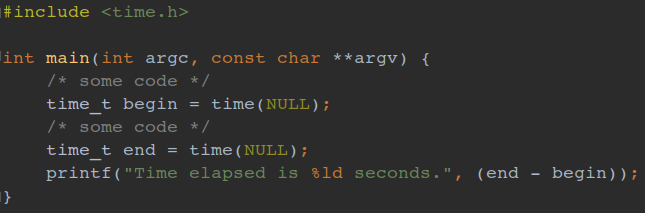
\includegraphics[width=0.8\textwidth]{images/image01.png}
  \label{fig:01}

  \caption{Código para geração do vetor randômico.}
  \centering
  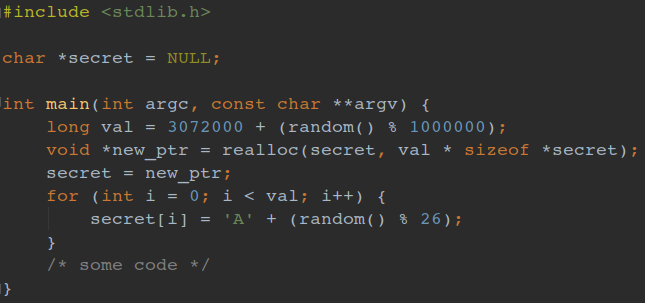
\includegraphics[width=0.8\textwidth]{images/image02.png}
  \label{fig:02}
\end{figure}

Antes de iniciar as modificações pontais, o \emph{exploit} foi adaptado para ter seu tempo de execução calculado, contando a partir do inicio da fase de treinamento (conforme a figura \ref{fig:01}). Após isto, a primeira modificação feita para este experimento, foi o aumento do tamanho da informação secreta no código do \emph{exploit}. Aumentado de 40 bytes, para um valor randômico entre 3072 e 4072 Kbytes (conforme a figura \ref{fig:02}). Este vetor de caracteres foi preenchido randomicamente, e submetido ao código do \emph{exploit} para inferência das variáveis. Espera-se que a memória cache deixe de armazenar os valores iniciais, e somente os valores finais possam ser inferidos.

Após a finalização deste experimento, conclui-se que, ao saber o ponteiro de inicio da variável que contém a informação secreta, e de posse do tamanho desta informação, é possível inferir todos os dados em uma velocidade de aproximadamente \textbf{5.46 KB/s} (3 MB em 562 segundos, para o ambiente em questão). Mesmo que a informação inferida seja maior que a memória cache. Isto porque, a transferência dos dados acontece com um endereço por vez. Cada endereço inferido passa por 3 fazes: treinamento (\emph{loop} que acontece 30 vezes), leitura (\emph{loop} de 256 vezes) e inferência da melhor leitura (\emph{loop} de 256 vezes). Sendo que, cada etapa ocorre 999 vezes, garantindo um \textbf{acurácia de 0,01\%} nos resultados, conforme \citeonline{Kocher2018spectre}.

% ---------------------------------
% VAZANDO A USER SPACE
% ---------------------------------
\subsection{T02 - A \emph{PoC} não limita-se aos endereços físicos do contexto}

Isto acontece pois, segundo \emph{Intrinsics Guide} da \emph{Intel}, a instrução \verb|_mm_clflush| é utilizada para limpar uma informação que se conhece o endereço, em todos os níveis da hierarquia da cache \cite{intel-iguide}. E para inferir os dados especulados o \emph{exploit} da \emph{Spectre} precisa fazer o ciclo de tentativa de acesso e limpeza da cache sucessivas vezes, inferindo o menor tempo de acesso para as informações coletadas.
\begin{verbatim}
Tentei criar um array de uint8T que é 1byte, com 32 000 posições, pra simular o tamanho da cache L1
ma os endereços virtuais são sempre diferentes... E o mmclflush sempre usa os virtuais pra acessar a TBL

E eu estou precisando limpar a cache L1 inteira. Mas não estou conseguindo via:
_mm_clflush (tentei com 1 array, variando em vários endereços e nada)
_builtin__clear_cache (tentei com um range grande de endereços e nada)
__clear_cache (tentei com outro range também e nada)
na documentação do mm_clflush, diz que ele só limpa endereços virtuais que passam pela TBL...
Ai tu passa o ponteiro pra variável que você quer limpar, ele acha a variável na TBL, e pega o endereço físico do cache na TBL. De lá, ele sai limpando todos os níveis de cache...    

clflush precisa do endereço físico da variável???
limpar a cache varrendo todos os endereços, e retirando os endereços que não estão mapeados, utilizando o mincore()
https://cs.adelaide.edu.au/~yval/Mastik/
https://www.phoronix.com/scan.php?page=news_item&px=Linux-Spectre-V2-Userspace

Desativa ASLR, pega o endereco estatico e testa
Mas é, ele descobriu o problema explorando vuln no JIT BPF


Não sei se conhece mas existem instruções não-temporais que são instruções que não usam o cache
Se a execução especulativa usar instruções não-temporais, o problema não teria acontecido
Não estou dizendo que a solução para o problema é o uso de instruções não-temporais. Citei para tentar ajudar no entendimento do problema.

https://www.wired.com/story/meltdown-spectre-bug-collision-intel-chip-flaw-discovery/

https://cyber.wtf/2017/07/28/negative-result-reading-kernel-memory-from-user-mode/

https://www.redhat.com/en/blog/understanding-mds-vulnerability-what-it-why-it-works-and-how-mitigate-it

https://news.ycombinator.com/item?id=18362905

https://arxiv.org/pdf/1902.05178.pdf
\end{verbatim}
Objetivo do teste
Descrição do teste (condição de execução)
Resultado do teste (empregar gráficos e tabelas, se possível)
Interpretação do resultado (discutir o resultado relacionando com a literatura)
Conclusão parcial do Teste 2

% ---------------------------------
% TENTANDO MAIS ALGUMA COISA
% ---------------------------------
\subsection{T03 - É imprescindível a utilização de \emph{Bit Twiddling}}
Objetivo do teste
Descrição do teste (condição de execução)
Resultado do teste (empregar gráficos e tabelas, se possível)
Interpretação do resultado (discutir o resultado relacionando com a literatura)
Conclusão parcial do Teste n

% ---------------------------------
% TENTANDO MAIS ALGUMA COISA
% ---------------------------------
\subsection{T04 - ???}
Objetivo do teste
Descrição do teste (condição de execução)
Resultado do teste (empregar gráficos e tabelas, se possível)
Interpretação do resultado (discutir o resultado relacionando com a literatura)
Conclusão parcial do Teste n

% ---------------------------------
% CONCLUSÃO DOS TESTES
% ---------------------------------
\subsection{Conclusão}

listar as condições necessárias pra explorar (listar os axiomas)
Síntese das conclusões parciais (Teste 1, Teste 2, ... Teste n)
Generalização dos resultados dos testes

% Finaliza a parte no bookmark do PDF, para que se inicie o bookmark na raiz
\bookmarksetup{startatroot}
% ------------------------------------------------------------------------
% CONCLUSÃO
% ------------------------------------------------------------------------
%\section{Considerações finais}
%\lipsum[31]
% ------------------------------------------------------------------------
% ELEMENTOS PÓS-TEXTUAIS
% ------------------------------------------------------------------------
\postextual
% ------------------------------------------------------------------------
% REFERẼNCIAS
% ------------------------------------------------------------------------
\bibliography{references}
% ------------------------------------------------------------------------
% APÊNDICES
% ------------------------------------------------------------------------
\begin{apendicesenv}
%\chapter{Cras non urna sed feugiat cum sociis natoque penatibus et magnis dis parturient montes nascetur ridiculus mus}
%\lipsum[31]
\end{apendicesenv}
% ------------------------------------------------------------------------
% ANEXOS
% ------------------------------------------------------------------------
\begin{anexosenv}
\vspace{\onelineskip}
%\chapter{Cras non urna sed feugiat cum sociis natoque penatibus et magnis dis parturient montes nascetur ridiculus mus}
%\lipsum[31]
\end{anexosenv}
% ------------------------------------------------------------------------
% AGRADECIMENTOS
% ------------------------------------------------------------------------
\section*{Agradecimentos}
%\lipsum[31]
% ------------------------------------------------------------------------
% FINAL DO DOCUMENTO
% ------------------------------------------------------------------------
\end{document}